\documentclass{article}
\usepackage[dvipsnames]{xcolor}
\usepackage[paperwidth=17cm, paperheight=2.5cm, margin = 0cm, top=0.5cm]{geometry}
\usepackage{amsmath}


\usepackage{pgf}
\usepackage{tikz}
\usetikzlibrary{positioning, calc}
\usetikzlibrary{arrows,automata}
\usetikzlibrary{arrows.meta}


\tikzstyle{bluebox} = 
[
	draw,rectangle,thick,inner sep=2mm,
	text width=2cm, minimum height=1.4cm,
	fill=blue, opacity=0.3, text opacity=1, draw opacity=1
]

\tikzstyle{thistlebox} = 
[
	draw,rectangle,thick,inner sep=2mm,
	text width=2cm, minimum height=1.4cm,
	fill=Thistle, text opacity=1, draw opacity=1
]

\tikzstyle{apricotbox} = 
[
	draw,rectangle,thick,inner sep=2mm,
	text width=2cm, minimum height=1.4cm,
	fill=Apricot, text opacity=1, draw opacity=1
]

\tikzstyle{whitebox} = 
[
	draw,rectangle,thick,inner sep=2mm,
	text width=2cm, minimum height=1.4cm,
	fill=white, text opacity=1, draw opacity=1
]

\renewcommand{\vec}[1]{\boldsymbol{#1}}

\begin{document}
\begin{center}
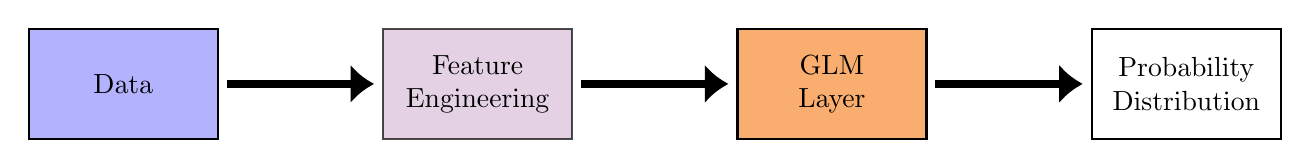
\begin{tikzpicture}[->,>=stealth',shorten >=1pt,auto,node distance=4.5cm,semithick]
\node[bluebox](X){\centerline{Data}};
\node[thistlebox, opacity=0.7](F1)[right of=X]{\centerline{Feature} \\\centerline{Engineering}};
\node[apricotbox](F2)[right of=F1]{\centerline{GLM} \\ \centerline{Layer}};
\node[whitebox](Y)[right of=F2]{\centerline{Probability}\\ \centerline{Distribution}};


\draw[-{Latex[length=3mm,width=5mm]}, line width=1mm, shorten <= 1mm, shorten >= 1mm] (X)--(F1);
\draw[-{Latex[length=3mm,width=5mm]}, line width=1mm, shorten <= 1mm, shorten >= 1mm] (F1)--(F2);
\draw[-{Latex[length=3mm,width=5mm]}, line width=1mm, shorten <= 1mm, shorten >= 1mm] (F2)--(Y);

\end{tikzpicture}
\end{center}

\end{document}
